%! Author = joaos
%! Date = 02/11/2024
\pagestyle{fancy}

\section*{Preparação e Caracterização de Amostras}

\newday{21 Outubro 2024}

Foi feito um trabalho de desagregação da amostra inicial, proveniente da mina do Numão.
Uma amostra de um pré-concentrado que tinha sido anteriormente submetida a processos de flutuação.
A amostra tinha cerca de 15~kg.

\begin{marginfigure}
    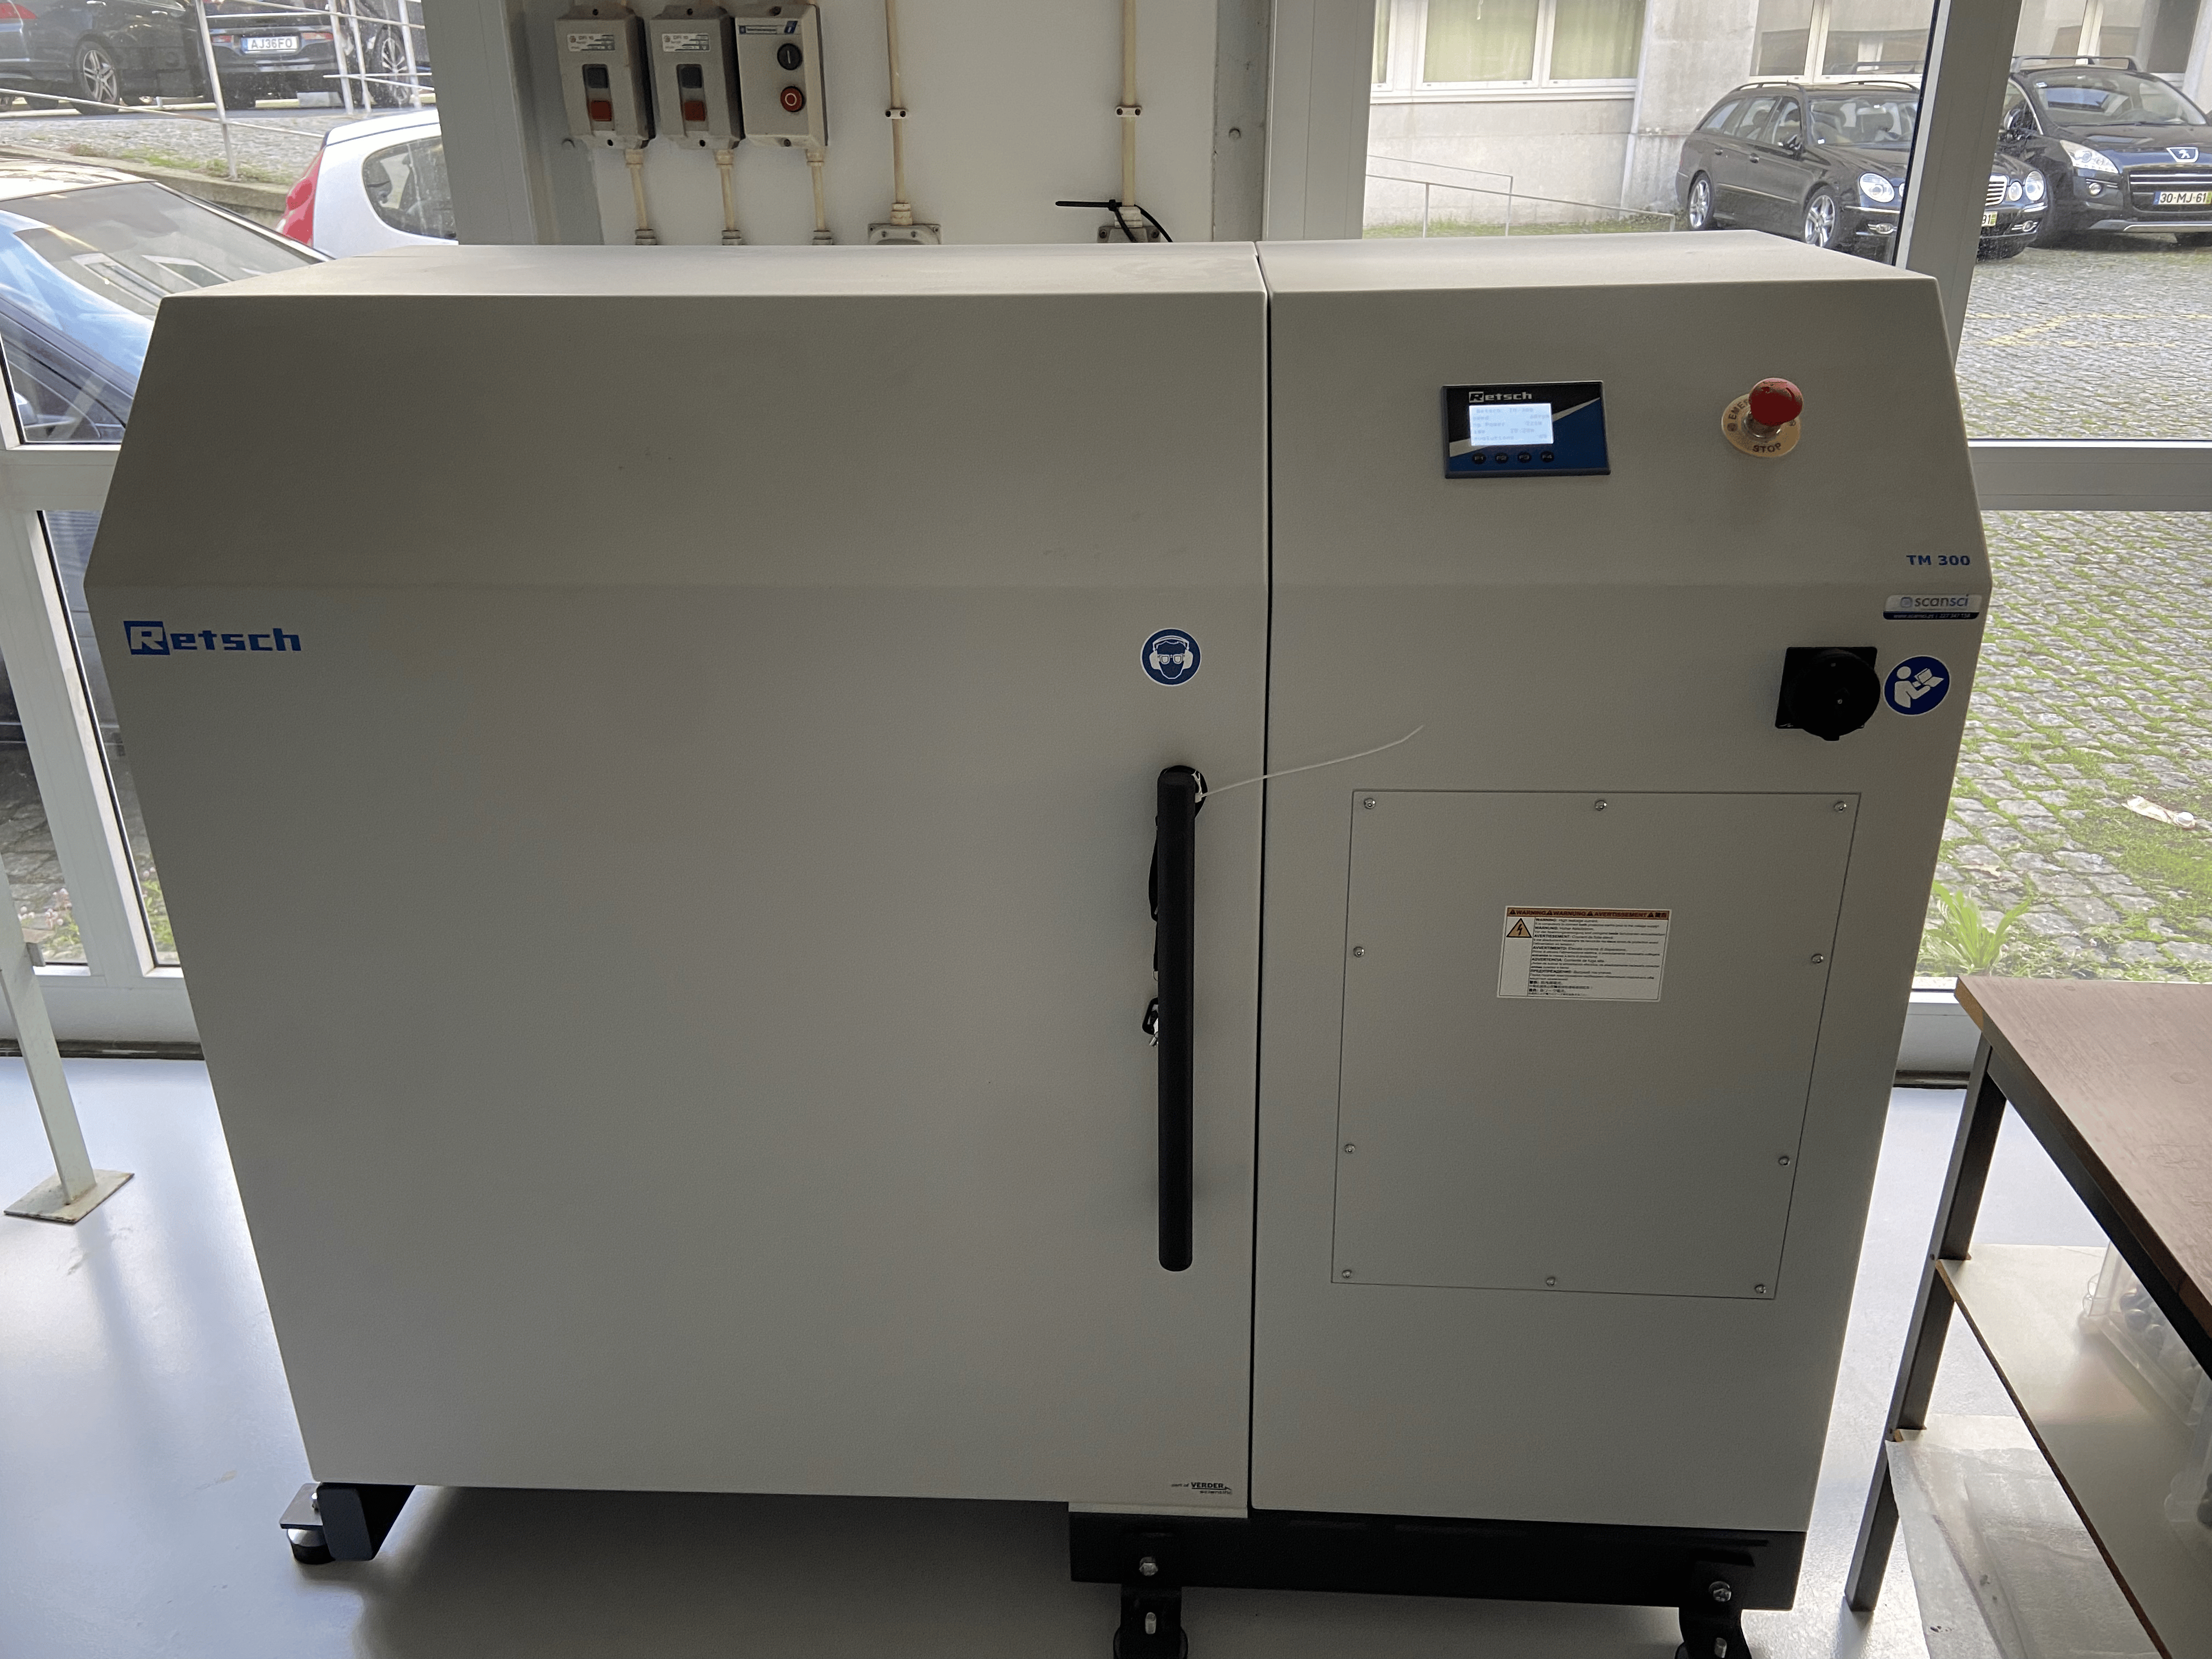
\includegraphics[width=\linewidth]{figures/moinho_tm300}
    \caption{Moinho de tambor \href{https://www.retsch.pt/pt/produtos/trituracao/moinhos-planetarios-e-de-bolas/tm-300/}{TM 300 Retsch}.}
    \label{fig:moinho_tm300}
\end{marginfigure}

Foi utilizado um moinho de bolas - apresentado na Figura~\ref{fig:moinho_tm300} - com a seguinte configuração de trabalho:
\begin{itemize}
    \item[-] 60 rpm;
    \item[-] Duração de trabalho 30~minutos;
\marginnote{Como o moinho nunca tinha sido utilizado para desagregar amostras, fez-se testes para determinar o tempo necessário de funcionamento e para determinar também a necessidade ou não de bolas.}
    \item[-] Sentido de rotação inverte de 5 em 5~minutos;
    \item[-] Pausa de 1~minuto entre cada inversão de sentido;
    \item[-] 3,41~kg de bolas.
\end{itemize}

Foi-se colocando partes da amostra dentro do tambor do moinho e deixou-se a desagregar durante o tempo estipulado.
\marginnote{O peneiro de \#1.18~mm foi utilizado como redundância, apenas para ter a certeza que toda a amostra estava desagregada.}
Uma vez terminado o tempo de funcionamento do moinho, peneirou-se o material desagregado com um peneiro de malha \#1.18~mm.
Foi-se fazendo este procedimento sucessivamente.
Deixou-se material para o dia seguinte.

\hrulefill

%%%%%%%%%%%%%%%%%%%%%%%%%%%%%%%%%%%%%%%%%%%%%%%%%%%%%%%%

\newday{22 Outubro 2024}

\textit{Na Figura~\ref{fig:amostra_no_moinho} temos a amostra de material dentro do tambor do moinho.}

\begin{marginfigure}[4\baselineskip]
    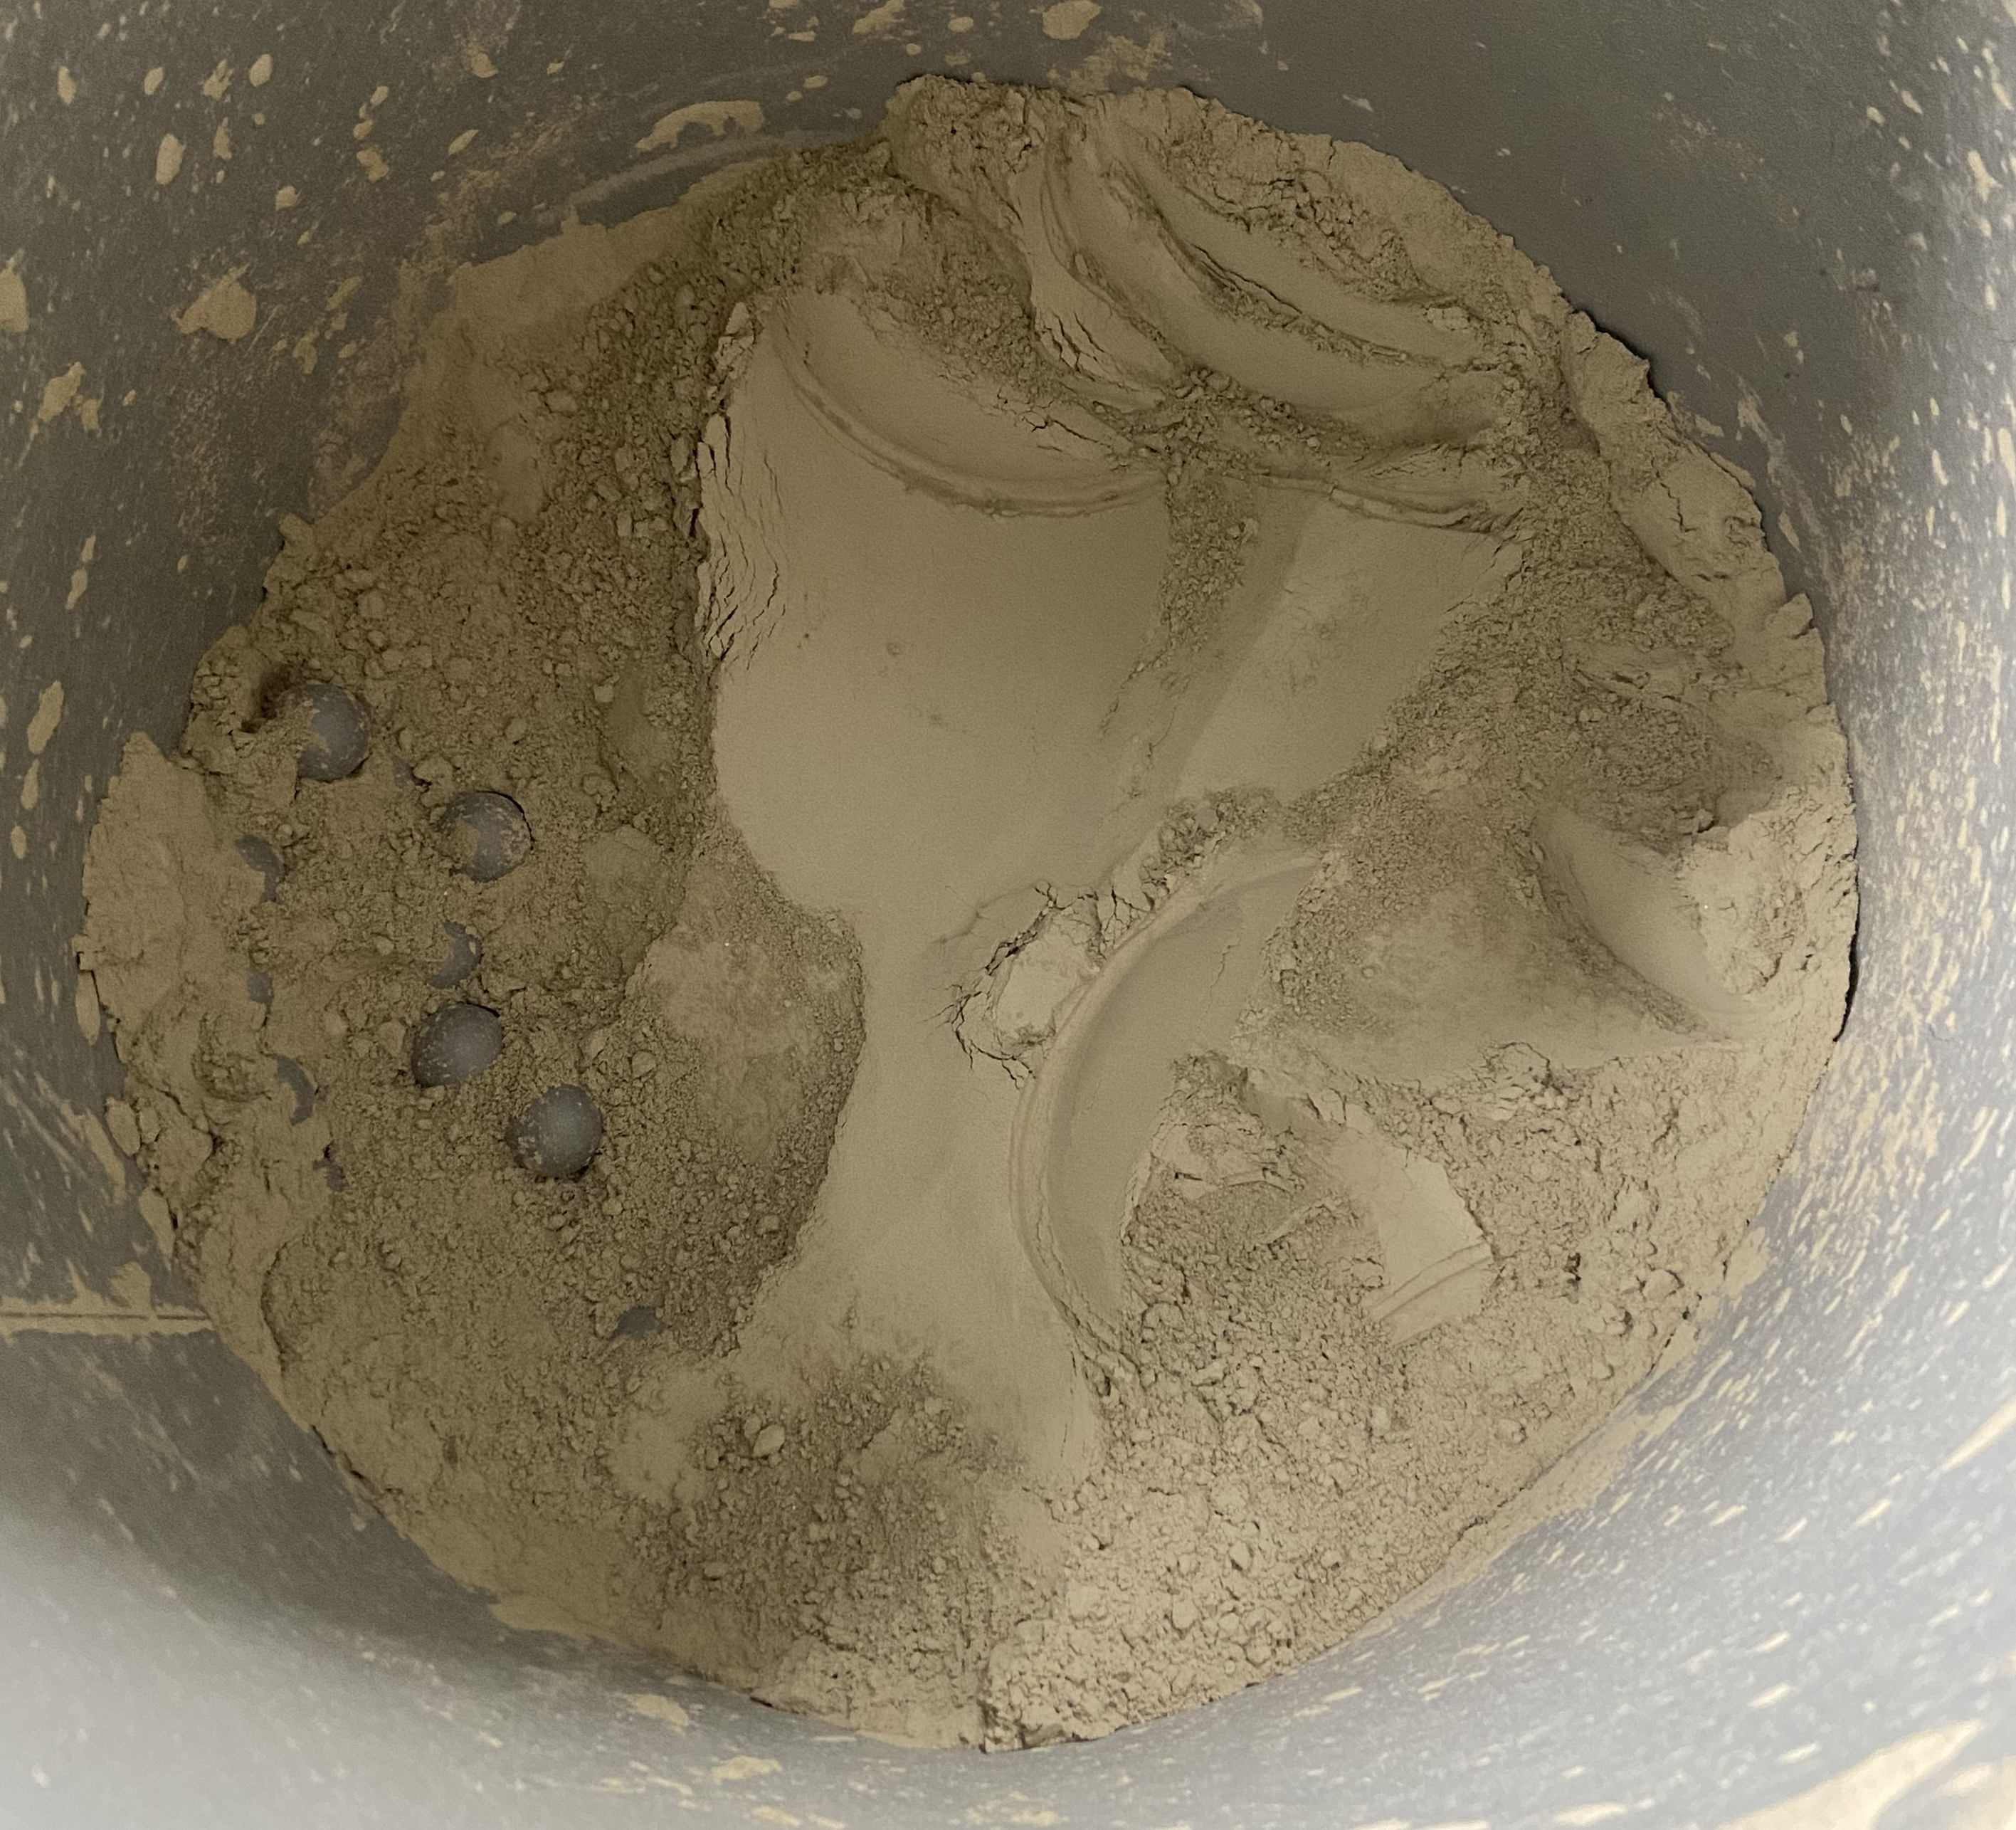
\includegraphics[width=0.9\linewidth]{figures/amostra_no_moinho}
    \caption{Amostra de material no tambor do moinho.}
    \label{fig:amostra_no_moinho}
\end{marginfigure}

Do dia anterior verificou-se que ainda havia alguns ``blocos'', portanto meteu-se o moinho a trabalhar durante cerca de 15~minutos para desagregar o resto do material.
Quando este terminou, a totalidade da amostra foi desagregada e peneirada com o peneiro \#1.18~mm.

Com o material já desagregado, era necessário agora homogeneizar a amostra.
Para isso, foi utilizado o separador \emph{Jones}\sidenote{O separador \emph{Jones}, ou em inglês \emph{riffle splitter}, é utilizado para separar amostras em duas partes quase idênticas.} (esquartelador).
Separou-se a amostra de $\approx$~15~kg em duas amostras de $\approx$~7,5~kg cada - amostra \texttt{A} e amostra \texttt{B}\@.

A amostra B vai ser guardada.
Foi armazenada em dois sacos de plástico - \texttt{B1} = 3,36~kg e \texttt{B2} = 4,28~kg.
A amostra \texttt{A} será posteriormente separada em sacos de $\approx$~1~kg.

\hrulefill
\pagebreak
%%%%%%%%%%%%%%%%%%%%%%%%%%%%%%%%%%%%%%%%%%%%%%%%%%%%%%%%

\newday{24 Outubro 2024}

\textit{N.B.: Antes de se utilizar o separador \emph{Jones}, tinha sido feita uma separação manual. Esta abordagem não poderia estar mais errada, separar a amostra manualmente introduz erros significativos, especialmente em amostras com partículas de diferentes calibres. O Jones é uma das formas representativas e precisas de separação de amostras e é o que será utilizado neste trabalho.}

\marginnote{É importante ter em consideração que obtêm-se sempre duas amostras com o separador \textit{Jones}, mas que uma das metades obtidas é \textbf{sempre} descartada. Ou seja, na Figura~\ref{fig:diagrama_jones}, o ramo da direita de cada uma das ramificações foi descartado para ser separado posteriormente (a totalidade da amostra foi separada em sacos de $\approx$~1~kg).}

\subsection{Funcionamento do separador Jones}\label{subsec:funcionamento-do-separador-jones}

O \emph{Jones} separa uma amostra em duas metades, sendo que uma das metades separadas é descartada e trabalha-se com a outra.

Um esquema de funcionamento desta separação está apresentado na Figura~\ref{fig:diagrama_jones}.

\begin{figure}[!ht]
    \centering
    \includegraphics[width=0.9\textwidth]{figures/diagrama_jones}
    \caption{Diagrama de separação de amostras com o Jones.}
    \label{fig:diagrama_jones}
\end{figure}

A amostra foi separada, com o separador \textit{Jones}, em sacos de aproximadamente 1~kg.
A massa de cada saco está apresentada na Tabela~\ref{tab:massa_sacos}.

\begin{table}[!htbp]
    \centering
    \begin{tabular}{@{}lc@{}}
        \toprule
        \textbf{Amostra} & \textbf{Massa (g)} \\ \midrule
        \textcolor{customblue}{A$_{01}$} & \textcolor{customblue}{1020,66} \\
        A$_{02}$ & 836,56 \\
        A$_{03}$ & 802,66 \\
        \textcolor{customorange}{A$_{04}$} & \textcolor{customorange}{1052,15} \\
        A$_{05}$ & 986,89 \\
        A$_{06}$ & 786,81 \\
        A$_{07}$ & 1138,15 \\
        \textcolor{customgreen}{A$_{08}$} & \textcolor{customgreen}{1044,50} \\ \midrule
        \textbf{Total} & 7590,38 \\ \bottomrule
    \end{tabular}
    \caption{Massa dos amostras separadas com o \emph{Jones}.}
    \label{tab:massa_sacos}
\end{table}

\marginnote[-0.5cm]{As células destacadas representam as amostras escolhidas para crivagem, que vai ser realizada posteriormente.}

\hrulefill

%%%%%%%%%%%%%%%%%%%%%%%%%%%%%%%%%%%%%%%%%%%%%%%%%%%%%%%%
\pagebreak

\newday{28 Outubro 2024}

Hoje foi realizada a crivagem do material previamente separado.
Escolheu-se, aleatoriamente, três dos oito sacos.
Os sacos escolhidos para crivagem foram os seguintes: \texttt{A01}, \texttt{A04} e \texttt{A08}; destacados na Tabela~\ref{tab:massa_sacos}.

A série de crivos utilizada para crivagem foi a seguinte:

\begin{minipage}{0.4\textwidth}
    \begin{enumerate}
        \item 0,850~mm
        \item 0,600~mm
    \end{enumerate}
\end{minipage}
\begin{minipage}{0.4\textwidth}
    \begin{enumerate}
        \setcounter{enumi}{2}
        \item 0,425~mm
        \item 0,300~mm
    \end{enumerate}
\end{minipage}

O material foi crivado nos crivos mecânicos\sidenote{Uma particularidade dos crivos mecânicos utilizados é que estes tinham a funcionalidade de definir automaticamente a frequência de vibração de acordo com o peso da coluna de crivos.} durante 30~minutos.
A mesma série de crivos foi utilizada para os três sacos.

Após cada crivagem, a massa das frações de material retido em cada um dos crivos da série de crivagem foi medida e está apresentada na Tabela~\ref{tab:massa_retido_crivagem}:

\begin{table}[!htb]
    \centering
    \begin{tabular}{@{}lccc@{}}
        \toprule
        \multirow{2}{*}{\textbf{Malha (mm)}} & \multicolumn{3}{c}{\textbf{Massa (g)}} \\ \cmidrule(lr){2-4}
         & \multicolumn{1}{c}{\textbf{A$\bm{_{01}}$}} & \multicolumn{1}{c}{\textbf{A$\bm{_{04}}$}} & \textbf{A$\bm{_{08}}$} \\ \hline
        \textbf{0,850} & \multicolumn{1}{c}{4,72} & \multicolumn{1}{c}{4,82} & 4,69 \\
        \textbf{0,600} & \multicolumn{1}{c}{4,26} & \multicolumn{1}{c}{4,48} & 4,43 \\
        \textbf{0,425} & \multicolumn{1}{c}{7,06} & \multicolumn{1}{c}{8,15} & 9,65 \\
        \textbf{0,300} & \multicolumn{1}{c}{30,65} & \multicolumn{1}{c}{31,53} & 41,93 \\
        \textbf{Infra} & \multicolumn{1}{c}{973,37} & \multicolumn{1}{c}{1002,44} & 982,95 \\ \midrule
        \textbf{\bm{$\sum$}}& \multicolumn{1}{c}{\textbf{1020,06}} & \multicolumn{1}{c}{\textbf{1051,42}} & \textbf{1043,65} \\ \bottomrule
    \end{tabular}
    \caption{Massa de material retido em cada crivo após a crivagem.}
    \label{tab:massa_retido_crivagem}
\end{table}

\newpara

Foi efetuada uma análise granulométrica do material retido em cada crivo.
A curva granulométrica está apresentada na Figura~\ref{fig:curva_granulometrica}.

\begin{figure}[!htb]
    \centering
    \begin{tikzpicture}[font=\footnotesize]
    \begin{axis}[
        xlabel={Crivo (mm)},
        ylabel={Cumulante Inferior (\%)},
        xmode=log,
        xtick={0.1, 1, 10},
        xticklabel style={/pgf/number format/fixed},
        log ticks with fixed point,
        xmin=0.1, xmax=10,
        ymin=93, ymax=100,
        ylabel near ticks,
        yticklabel=\pgfmathprintnumber{\tick},
        width=10cm,
        height=8cm,
        grid=both,
        grid style={dashed, gray!30},
        enlarge x limits={abs=0.5cm},
        axis lines= left,
        legend pos=south east,
        height=6.5cm,
    ]
    % Série A01
    \addplot[
        mark=*,
        mark options={scale=1, fill=customblue},
        color=customblue,
        line width=0.7pt
    ] coordinates {
        (1.18, 100.00)
        (0.850, 99.54)
        (0.600, 99.12)
        (0.425, 98.43)
        (0.300, 95.42)
    };
    \addlegendentry{A01}

    % Série A04
    \addplot [
        mark=*,
        mark options={scale=1, fill=customorange},
        color=customorange,
        line width=0.7pt
    ] coordinates {
        (1.18, 100.00)
        (0.850, 99.54)
        (0.600, 99.12)
        (0.425, 98.34)
        (0.300, 95.34)
    };
    \addlegendentry{A04}

    % Série A08
    \addplot[
        mark=*,
        mark options={scale=1, fill=customgreen},
        color=customgreen,
        line width=0.7pt
    ]  coordinates {
        (1.18, 100.00)
        (0.850, 99.55)
        (0.600, 99.13)
        (0.425, 98.20)
        (0.300, 94.18)
    };
    \addlegendentry{A08}

    \end{axis}
    \end{tikzpicture}
    \caption{Curva granulométrica.}
    \label{fig:curva_granulometrica}
\end{figure}

Como existe muito pouco material acima do calibre 0,300~mm (<~5~\%), juntou-se todas as frações de material novamente e vai-se realizar medições no granulómetro laser.

\hrulefill
\pagebreak
%%%%%%%%%%%%%%%%%%%%%%%%%%%%%%%%%%%%%%%%%%%%%%%%%%%%%%%%

\newday{30 Outubro 2024}

\newthought{Granulómetro Laser} \href{https://www.malvernpanalytical.com/en/support/product-support/mastersizer-range/mastersizer-2000}{Malvern Mastersizer 2000}

\marginnote{Um granulómetro laser utiliza a difração da luz laser para medir a distribuição dos tamanhos das partículas numa amostra. Este tipo de análise é particularmente útil porque permite uma análise rápida, precisa e repetível.}

Continuando o trabalho, as frações das amostras previamente crivadas foram colocadas todas na sua forma original (amostra tal-qual de $\approx$~1~kg) para se analisar a granulometria dos 8~sacos de material, com auxílio do granulómetro laser - Figura~\ref{fig:granulometro_laser}.

\begin{figure}[!htb]
    \centering
    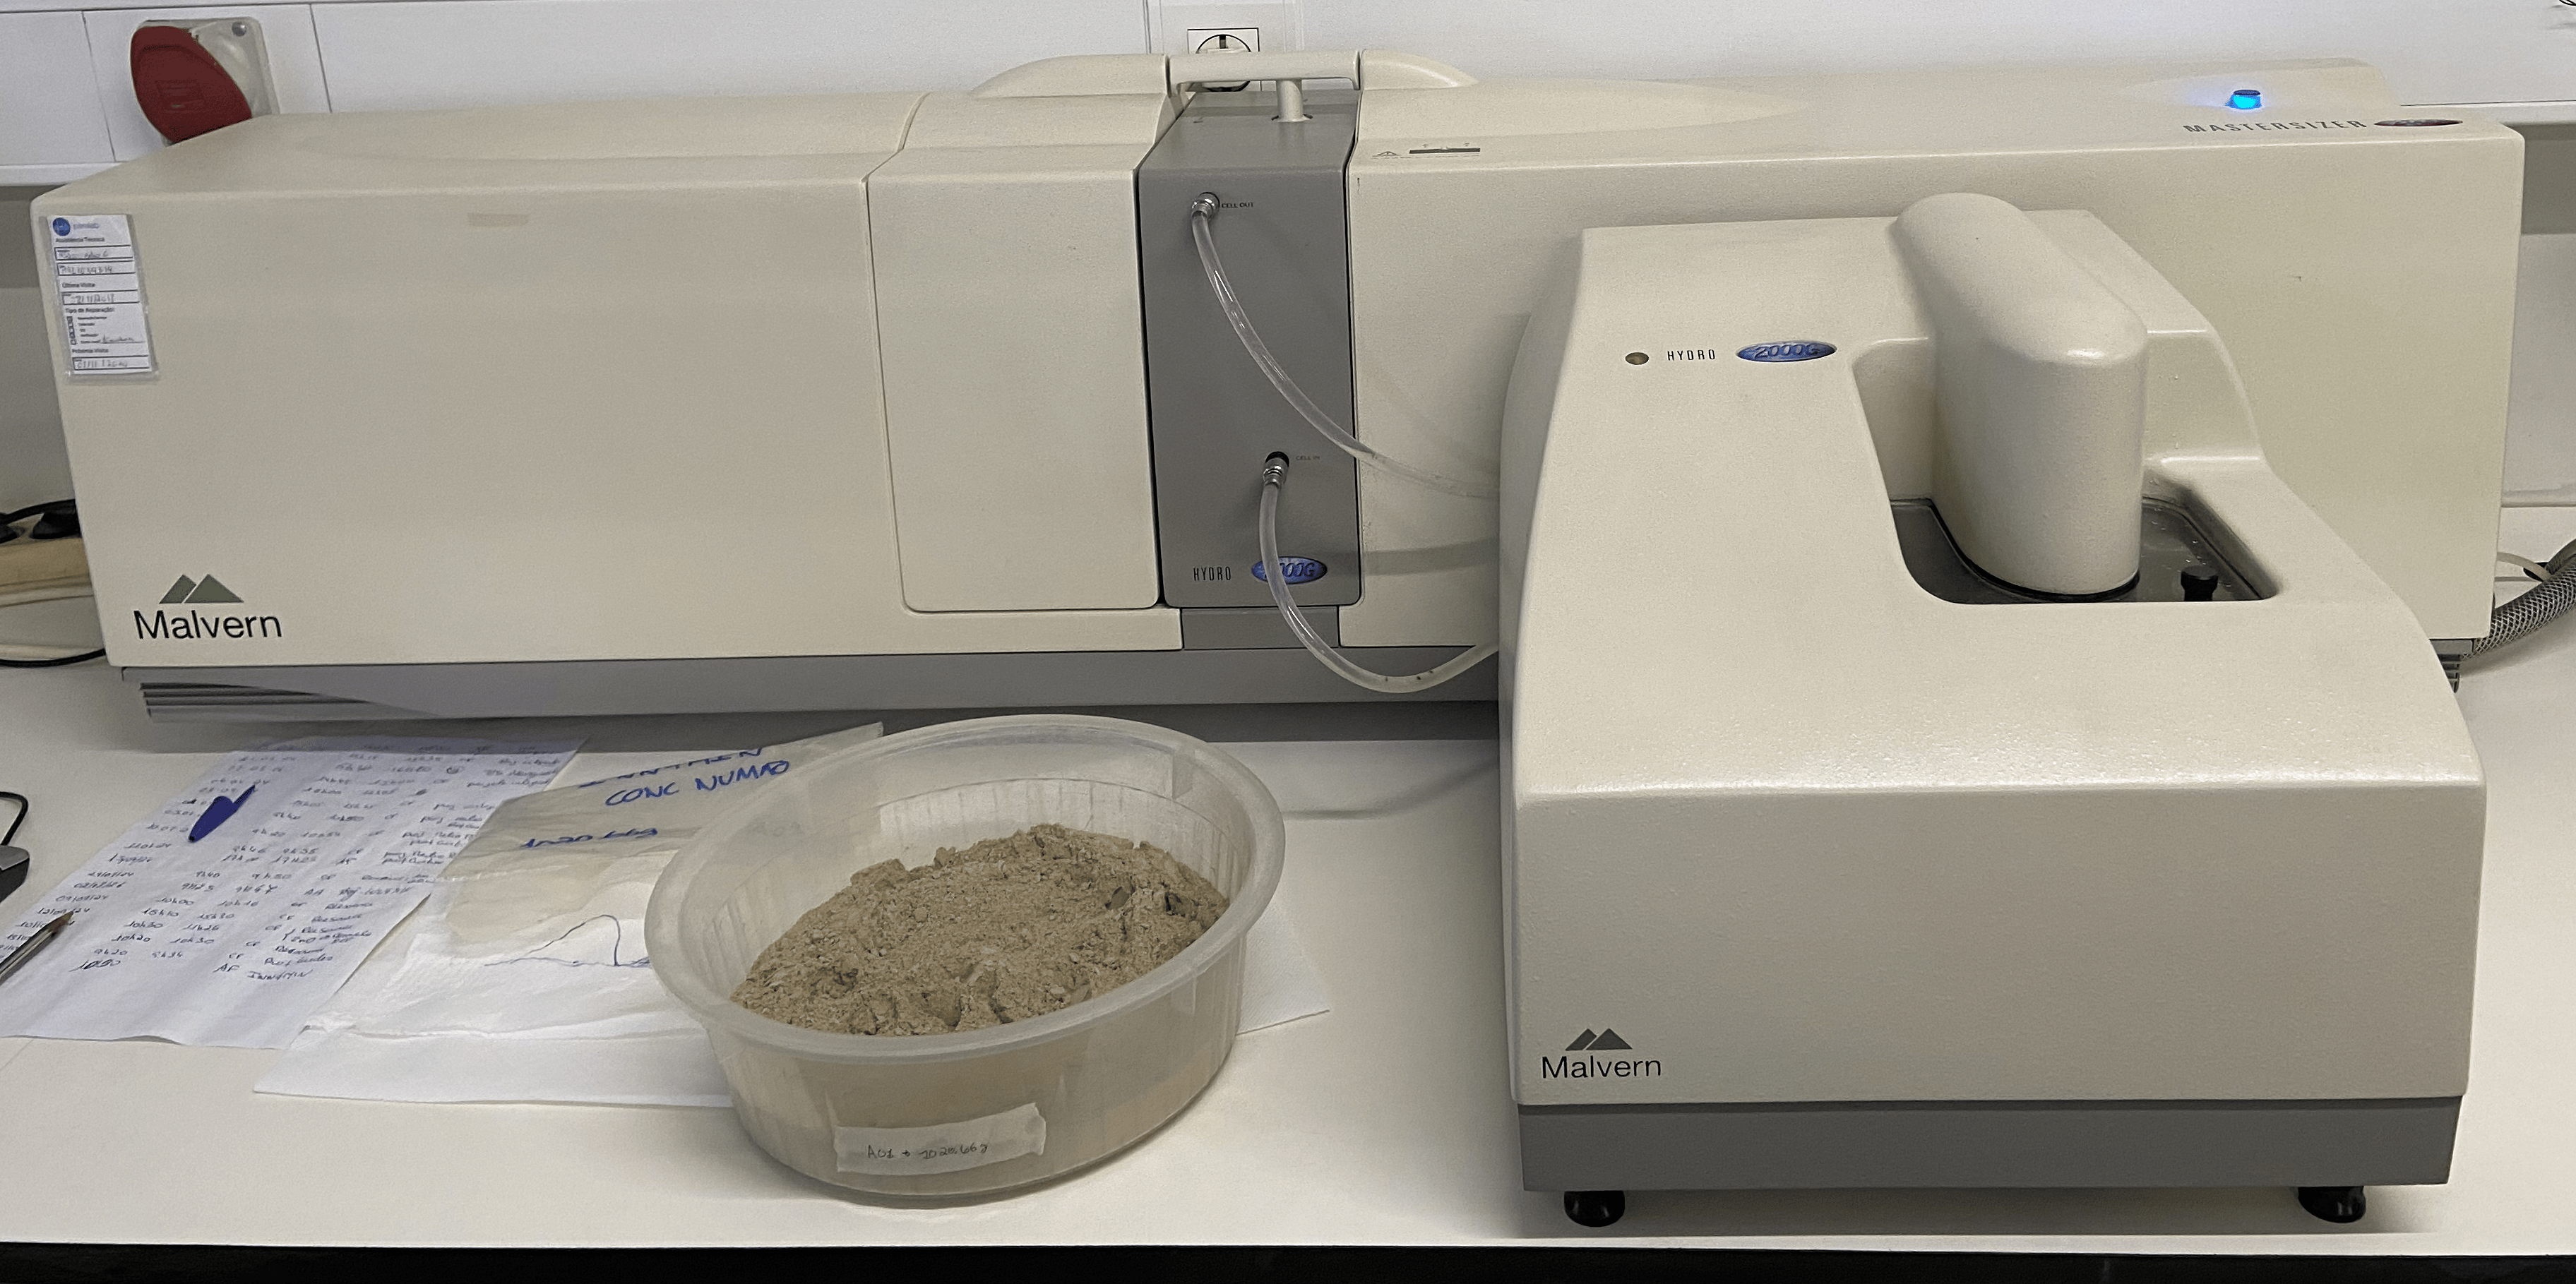
\includegraphics[width=0.75\linewidth]{figures/granulometro_laser}
    \caption{Granulómetro laser Malvern Mastersizer 2000.}
    \label{fig:granulometro_laser}
\end{figure}

Começou-se por analisar a amostra \texttt{A01}\sidenote[][-0.25cm]{As amostras foram analisadas separadamente, mas com os resultados obtidos de todas as subamostras poderemos generalizar para a amostra tal-qual ($\approx$~15~kg).}.
A primeira análise foi feita com a amostra seca (ou seja, foi colocada no granulómetro sem estar misturada em água), de forma a avaliar a distribuição do tamanho das partículas.
Verificou-se que havia partículas ainda agregadas\sidenote{Como estamos a trabalhar com material de calibre muito fino, é normal haver agregação de partículas. Isto pode ser combatido com uma agitação forte; uso de ultra-som ou mistura prévia em água para desagregar.}.

Limpou-se o granulómetro e fez-se outra análise desta vez tendo misturado a amostra em água para evitar a agregação das partículas.
Mesmo assim, era possível melhorar ainda mais os resultados e portanto utilizou-se a opção de ultra-som para promover ainda mais a desagregação das partículas.

Visto que com uma mistura prévia em água e com a utilização da opção de ultra-som do granulómetro obtiam-se os melhores resultados, os restantes sacos foram analisados com estas parametrizações.
Sendo que, antes de se ativar o ultra-som\sidenote{A utilização do ultra-som, se for possível, deve ser evitada pois como as partículas são muito finas pode promover a fragmentação e resultar em análises erradas que não refletem a verdadeira composição da amostra.} realizou-se sempre uma análise apenas com a mistura prévia em água.

As análises foram identificadas da seguinte forma:
\begin{itemize}
    \item[-] \texttt{A0n}, sendo \texttt{n} o número da amostra, para análises sem mistura prévia em água e sem ultra-som;
    \item[-] \texttt{A0n-REP}, para análise com mistura prévia em água e sem ultra-som;
    \item[-] \texttt{A0n-REP2}, para análise com mistura prévia em água e com ultra-som.
\end{itemize}

\marginnote[-0.5cm]{Para cada análise foram guardados ficheiros distintos com uma curva granulométrica e com uma curva de distribuição de calibres, \texttt{A0n-REP2-CUM} e \texttt{A0n-REP2-FREQ}, respetivamente.}

Os dados das análises foram guardados para uso posterior.

\hrulefill
\pagebreak

%%%%%%%%%%%%%%%%%%%%%%%%%%%%%%%%%%%%%%%%%%%%%%%%%%%%%%%%

\newday{31 Outubro 2024}\label{day:31-outubro-2024}

\begin{marginfigure}[3\baselineskip]
    \centering
    \includegraphics[width=0.55\linewidth]{figures/divisor_de_amostras_retsch}
    \caption{Divisor de amostras \href{https://www.retsch.pt/pt/produtos/assistencia/amostradores/pt-100/}{PT 100}.}
    \label{fig:divisor_de_amostras_retsch}
\end{marginfigure}

Uma fez realizada a análise granulométrica no granulómetro laser, iremos dar continuação à amostragem.
O próximo passo será dividir as amostras de 1~kg em sub-amostras de, aproximadamente 0,250~g - deveremos ter no máximo 250~g e no mínimo 200~g.

Para esta divisão foi utilizado o divisor de amostras apresentado na Figura~\ref{fig:divisor_de_amostras_retsch}.
Este equipamento em específico, divide a amostra em 8~partes iguais.
Portanto, das nossas amostras de $\approx$~1~kg iremos obter 8 sub-amostras de $\approx$~0,125~kg.
Como queremos que as nossas sub-amostras tenham $\approx$~0,250~kg, iremos juntar os frascos resultantes da divisão 2~a~2.

O funcionamento do divisor de amostras é bastante simples e direto.
Coloca-se os frascos, liga-se o equipamento, liga-se o alimentador e coloca-se a amostra (pouco a pouco para prevenir entupimentos) no funil do alimentador\sidenote{O divisor de amostras conta com o alimentador \href{https://www.retsch.pt/pt/produtos/assistencia/alimentadores/}{DR 100} que promove a alimentação contínua de material ao divisor.}.
O divisor faz o resto do trabalho, dividindo a amostra em 8~sub-amostras praticamente iguais.

Das 8~sub-amostras obtidas em cada uma das divisões, constitui-se sacos de $\approx$~0,250~kg, juntando os frascos 2~a~2.
As massas de cada uma das sub-amostras está apresentada na tabela seguinte:

\begin{table*}[ht]
\centering
    \begin{tabular}{@{}lcccccccc@{}}
        \toprule
        \textbf{Sub-amostras (g)} & \textbf{A\bm{$_{01}$}} & \textbf{A\bm{$_{02}$}} & \textbf{A\bm{$_{03}$}} & \textbf{A\bm{$_{04}$}} & \textbf{A\bm{$_{05}$}} & \textbf{A\bm{$_{06}$}} & \textbf{A\bm{$_{07}$}} & \textbf{A\bm{$_{08}$}} \\ \hline
        \textbf{A\bm{$_{0\text{n.}1}$}} & 254,44 & 207,90 & 200,00 & 262,99 & 243,20 & 196,06 & 283,14 & 264,14 \\
        \textbf{A\bm{$_{0\text{n.}2}$}} & 253,67 & 208,76 & 202,18 & 262,30 & 245,76 & 192,84 & 286,50 & 260,05 \\
        \textbf{A\bm{$_{0\text{n.}3}$}} & 254,76 & 210,29 & 200,52 & 262,23 & 250,16 & 198,40 & 284,01 & 257,18 \\
        \textbf{A\bm{$_{0\text{n.}4}$}} & 254,22 & 209,50 & 198,21 & 262,28 & 246,06 & 198,43 & 282,14 & 259,72 \\ \midrule
        \textbf{\bm{$\sum$}} & 1017,09 & 836,45 & 800,91 & 1049,80 & 985,18 & 785,73 & 1135,79 & 1041,09 \\ \bottomrule
    \end{tabular}
\end{table*}

\newpara

Uma vez divididas as sub-amostras, iremos escolher um dos sacos de $\approx$~250~g proveniente da divisão de cada um dos 8 sacos de $\approx$~1~kg.
Estas 8 sub-amostras irão ser analisadas no FRX\sidenote{A fluorescência de raios X (FRX) é uma técnica rápida e não destrutiva amplamente usada para determinar a composição elementar de um material que requer apenas uma preparação mínima da amostra.} para determinar a composição química das amostras.
Como o teor em \ce{Au} deve ser muito pequeno, ele não será determinado por esta análise, obteremos apenas os elementos em maior quantidade.

Foram escolhidas as amostras \texttt{A01.1}, \texttt{A02.3}, \texttt{A03.2}, \texttt{A04.3}, \texttt{A05.3}, \texttt{A06.4}, \texttt{A07.4} e \texttt{A08.3} para serem analisadas no FRX\@.

\begin{marginfigure}[1\baselineskip]
    \centering
    \includegraphics[width=0.7\linewidth]{figures/FRX}
    \caption{Equipamento FRX utilizado.}
    \label{fig:equipamento_frx}
\end{marginfigure}

O funcionamento do equipamento FRX é bastante simples, basta colocar a amostra dentro do equipamento, fechar bem a porta e acionar o gatilho para começar a análise.
Foram realizados cinco ``tiros'' por amostra, com um tempo de análise de 30~segundos em cada tiro.
No fim de cada tiro, foi-se alterando a posição da amostra dentro do equipamento, para que fossem analisadas diferentes partes da amostra de forma a que os resultados sejam representativos.

Os resultados das análises foram descarregados em formato \texttt{.csv}.
Os dados irão ser posteriormente analisados.

%%%%%%%%%%%%%%%%%%%%%%%%%%%%%%%%%%%%%%%%%%%%%%%%%%%%%%%%

\newday{6 Novembro 2024}

Hoje foram refeitas as análises FRX para as amostras \texttt{A01.1}, \texttt{A03.2}, \texttt{A05.3} e \texttt{A08.3}.
Os valores destas análises serão adicionados (substituídos) aos dados obtidos no dia~\nameref{day:31-outubro-2024}.

A necessidade de refazer as análises para estas amostras assenta no facto de o equipamento não ter feito leituras de alguns elementos em alguns dos 5~tiros realizados.
Portanto, é necessário refazer a análise FRX para estas amostras para que a média, que vai ser calculada, seja correta e que os resultados sejam representativos.

\hrulefill
%%%%%%%%%%%%%%%%%%%%%%%%%%%%%%%%%%%%%%%%%%%%%%%%%%%%%%%%

\newday{7 Novembro 2024}\label{day:7-novembro-2024}

Hoje foi feita a preparação para fazer a digestão ácida\sidenote{A digestão ácida serve para decompor a matriz mineral da amostra, permitindo a solubilização dos elementos de interesse (neste caso, o ouro e possivelmente outros metais associados) e eliminando interferências que poderiam afetar a análise subsequente por espectrometria de absorção atómica.}.
Para isso foi escolhida, aleatoriamente, uma sub-amostra de $\approx$~250~g para este procedimento.
Foi escolhida a amostra \texttt{A08.3}, com 257,18~g.

Como vão ser necessários apenas 50~g de amostra, a \texttt{A08.3} foi colocada no divisor de amostras - o mesmo da Figura~\ref{fig:divisor_de_amostras_retsch}.

Do divisor de amostras obteu-se 54,15~g (\texttt{A08.3.1}) que foi depois dividido em cinco copos, cada um com aproximadamente 10~g.
Estes cinco copos foram depois colocados na mufla.
A mufla foi programada para aquecer até 700~\graus, manter os 700~\graus \, durante 1~hora e depois desligar-se automaticamente.
As amostras ficam a arrefecer dentro da mufla até ao dia seguinte.
\begin{marginfigure}[1\baselineskip]
    \centering
    \includegraphics[width=0.7\textwidth]{figures/Mufla}
    \caption{Mufla utilizada para aquecer a amostra.}
    \label{fig:mufla}
\end{marginfigure}

A amostra \texttt{A08.3} foi reconstituída com o material que não foi para os copos da mufla e foi medida a massa: 215.03~g (com o peso do saco).

No dia seguinte, com a amostra já arrefecida, será realizada a digestão ácida, sendo que o procedimento será posteriormente explicado.

\hrulefill

%%%%%%%%%%%%%%%%%%%%%%%%%%%%%%%%%%%%%%%%%%%%%%%%%%%%%%%%

\newday{8 Novembro 2024}\label{day:8-novembro-2024}

Retiraram-se as amostras que foram colocadas na mufla no dia~\nameref{day:7-novembro-2024}.
O material, anteriormente com uma cor beje (como se pode ver na Figura~\ref{fig:amostra_no_moinho}), encontra-se agora com uma cor avermelhada - Figura~\ref{fig:amostra-apos-mufla}.
\begin{marginfigure}[-3\baselineskip]
    \centering
    \includegraphics[width=0.9\linewidth]{figures/Amostra após mufla}
    \caption{Amostra após mufla a 700\graus.}
    \label{fig:amostra-apos-mufla}
\end{marginfigure}

O material foi transferido para gobelés brancos para serem submetidos à digestão ácida.
A digestão será feita com ácido nítrico, \ce{HNO_3}; e com ácido clorídrico, \ce{HCl}.
A relação vai ser de 1:3, ou seja, 6~ml de \ce{HNO_3} para 18~ml de \ce{HCl}, a 200~\graus.

A quantidade específicada de cada ácido é colocada em cada um dos 5~copos da Figura~\ref{fig:amostra-a-ser-atacada}, deixando a reação decorrer durante 1~hora e 30~minutos.
Serão feitos 3~ataques, ou seja, após cada hora e meia será colocado de novo ácido nítrico e ácido clorídrico.
Repete-se esta operação três vezes, totalizando em 4~horas e 30~minutos de reação.
\begin{marginfigure}[\baselineskip]
    \centering
    \includegraphics[width=0.9\linewidth]{figures/Amostra a ser atacada - digestão ácida}
    \caption{Amostra a ser atacada com ácido.}
    \label{fig:amostra-a-ser-atacada}
\end{marginfigure}

Após o terceiro e último ataque, foram adicionados 4~ml de \ce{HCl} a cada um os copos.
É necessário agora transferir o material dissolvido e separá-lo dos resíduos.
Para isso, com o auxílio de uma pinça, retirou-se o copo da areia, agitou-se um pouco o líquido no interior e transferiu-se cuidadosamente para um balão volumétrico de 50~ml tendo cuidado para parar de verter quando a cor do líquido passar de laranja para um verde acinzentado (o material verde acinzentado é o resíduo).
O restante volume do balão volumétrico foi preenchido com água destilada.

O resíduo foi colocado numa placa de Petri.
Colocou-se um pouco de água destilada no copo para facilitar a transferência do resíduo para a placa.
Fez-se isto para cada um dos 5~copos, resultando nas amostras apresentadas na Figura~\ref{fig:amostra-apos-digestao}.

\begin{marginfigure}[-3\baselineskip]
    \centering
    \includegraphics[width=0.8\linewidth]{figures/Amostra após Digestão}
    \caption{Amostra após a digestão.}
    \label{fig:amostra-apos-digestao}
\end{marginfigure}

Posteriormente será feita a filtragem do licor e do resíduo, do material presente nos balões volumétricos, para depois se proceder à absorção atómica.
Ainda será decidido o que será feito ao resíduo, pode possívelmente ser descartado.

\hrulefill

%%%%%%%%%%%%%%%%%%%%%%%%%%%%%%%%%%%%%%%%%%%%%%%%%%%%%%%%

\newday{12 Novembro 2024}

Hoje realizou-se a filtração do material proveniente da digestão ácida realizada no dia~\nameref{day:8-novembro-2024}.
Para isso utilizou-se um Kitsato\footnote{O balão kitsato é um tipo de vidraria de laboratório. Normalmente usado com um filtro de Büchner em filtrações em vácuo.}, um filtro de membrana e o porta-filtro (não me recordo no nome).
Este sistema foi conectado a uma bomba para se realizar a filtração em vácuo.

Foram colocadas as amostras da Figura~\ref{fig:amostra-apos-digestao}, cuidadosamente, no sistema de filtração, agitando o balão volumétrico para que o resíduo que estava depositado no fundo e o líquido se misturassem.

Foram realizadas duas filtrações para cada amostra.

O resíduo sólido foi separado para uma placa de Petri.
As amostras líquidas foram armazenadas para se realizar a absorção atómica e os resíduos foram embrulhados em Parafilm.

\hrulefill

\newthought{Fora do Laboratório} decidiu-se fazer um estudo prévio dos conceitos teóricos relativos à absorção atómica, para que, na altura de efetuar a análise, os conhecimentos básicos estejam consolidados e que se perceba o funcionamento do equipamento.

\subsection*{Espetroscopia}\label{subsec:espetroscopia}

Antes de falarmos sobre absorção atómica, devemos ter em consideração o conceito de espetroscopia.
A espetroscopia é a interação entre radiação\sidenote{O termo radiação, em física, apenas significa a propagação de energia de um ponto a outro. Por vezes este termo é usado comumente com outra conotação.} e matéria.
Isto acontece, quando os eletrões absorvem uma quantidade discreta de energia que os faz transitar, ou excitar, para órbitas atómicas de maior energia.
A energia que é absorvida pelos eletrões é sempre igual à diferença de energia entre as orbitas de transição.

É importante ter em consideração que órbitas de diferentes elementos têm níveis de energia diferentes.
Isto faz com que a quantidade de energia que é absorvida pelos eletrões seja também diferente para diferentes elementos.
Quando os eletrões excitados voltam para a sua orbita original, vão emitir a mesma quantidade de energia que foi previamente absorvida, sob a forma de radiação eletromagnética\sidenote{Radiação eletromagnética, ou REM, pode ser classificada de acordo com a sua frequência, a partir da qual diferentes comprimentos de onda estão associados, nas seguintes faixas: ondas de rádio, micro-ondas, radiação terahertz, radiação infravermelha, luz vísivel, radiação ultravioleta, raios X e radiação gama.}.

Sendo assim, como a quantidade de energia \textbf{absorvida} varia para diferentes elementos, a quantidade de energia \textbf{emitida} também varia para diferentes elementos.

\subsection*{Espetroscopia de absorção Atómica}\label{subsec:absorcao-atomica}

A espetroscopia de absorção atómica\sidenote{Ou AAS, do inglês \emph{Atomic Absorption Spectroscopy.}}, ou apenas absorção atómica, é uma técnica quantitativa que analisa a concentração de iões metálicos numa amostra, pelo uso de espetroscopia.

\begin{marginfigure}
    \centering
    \includegraphics[width=0.8\linewidth]{figures/Diagrama - espetroscopia}
    \caption{Transição de eletrões para diferentes níveis de energia.}
    \label{fig:diagrama-espetroscopia}
\end{marginfigure}

Os eletrões nos iões e átomos metálicos podem absorver REM para transitarem para órbitas de maior energia, como demonstrado na Figura~\ref{fig:diagrama-espetroscopia}.
A absorção atómica baseia-se no facto de que a quantidade de iões metálicos determina a quantidade de energia que é absorvida.
Mais iões metálicos existentes, maior a absorção de energia.

A absorção atómica é uma técnica extremamente sensível, pois é capaz de determinar e medir a presença de espécies metálicas através da quantidade de REM absorvida, mesmo em amostras com uma quantidade mínima de metal.

A relação entre a quantidade de iões metálicos ou de átomos presentes numa amostra e a quantidade de radiação que é absorvida é dada pela Lei de Beer-Lambert\sidenote[][-1.30cm]{A Lei de Beer-Lambert, também conhecida como Lei de Beer ou Lei de Beer-Lambert-Bouguer é uma relação empírica que, na ótica, relaciona a absorção de luz com as propriedades do material atravessado por ela.}, que diz que a quantidade de REM absorvida é \textbf{diretamente proporcional} à concentração de iões metálicos ou átomos.
Ou seja, se a concentração de iões metálicos ou átomos for baixa a absorção de energia também será baixa; se a concentração for alta a absorção de energia também será alta.
Assim, muito resumidamente, ao medir a quantidade de REM que é absorvida é possível calcular a concentração de um metal em específico.

\hrulefill
%%%%%%%%%%%%%%%%%%%%%%%%%%%%%%%%%%%%%%%%%%%%%%%%%%%%%%%%%

\newday{13 Novembro 2024}

Hoje efetuou-se a absorção atómica.
O equipamento utilizado foi o da Figura~\ref{fig:equipamento-absorcao-atomica}.

\begin{marginfigure}[8\baselineskip]
    \centering
    \includegraphics[width=0.95\linewidth]{figures/Absorção atómica}
    \caption{Equipamento para AAS (\href{https://www.analytik-jena.com/products/chemical-analysis/elemental-analysis/aas/zeenit-series/}{Analytik Jena ZEEnit 700P Furnace Vision}).}
    \label{fig:equipamento-absorcao-atomica}
\end{marginfigure}

É necessário fazer uma preparação prévia do equipamento para se realizar a análise, cerca de uma ou duas horas deve ser suficiente.
Os procedimentos necessários para o funcionamento correto do equipamento são bastante extensos e portanto não serão aqui abordados, no entanto deixa-se aqui \href{https://www.analytik-jena.com/fileadmin/import/assets/0000006182_Manual_ZEEnit_700_P_en.pdf}{o manual de funcionamento}.
Também existe um guia de manuseamento, bastante detalhado, disponível no laboratório.

Foi realizada uma curva de calibração, com soluções padrão de diferentes concentrações em \ce{Au}, desde 2~ppm a 10~ppm.
A curva está apresentada na Figura~\ref{fig:curva-calibracao-aas}.

\begin{figure}[!htb]
    \centering
    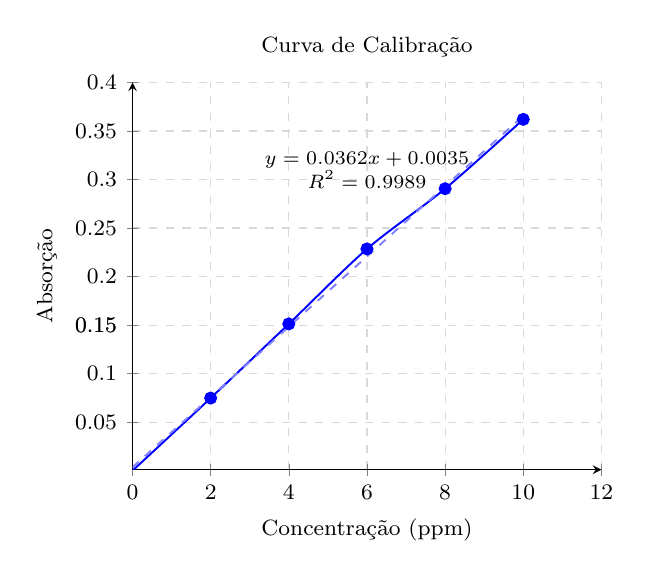
\begin{tikzpicture}[font=\footnotesize]
        \begin{axis}[
            title={Curva de Calibração},
            xlabel={Concentração (ppm)},
            ylabel={Absorção},
            xmin=0.001, xmax=12,
            ymin=0.001, ymax=0.4,
            ytick={0.05, 0.1, 0.15, 0.15, 0.2, 0.25, 0.30, 0.35, 0.40},
            yticklabel style={/pgf/number format/fixed},
            height=6.5cm,
            grid=major,
            grid style={dashed,gray!30},
            axis lines=left,
            legend pos=south east
        ]

        % Dados da tabela com linha suave entre pontos
        \addplot[
            mark=*,
            mark options={scale=1, fill=blue},
            color=blue,
            smooth,
            line width=0.7pt
        ] coordinates {
            (0, 0)
            (2, 0.07481)
            (4, 0.15123)
            (6, 0.22843)
            (8, 0.2905)
            (10, 0.36194)
        };

        % Linha de tendência (regressão linear)
        \addplot[
            domain=0:10,
            samples=100,
            color=blue!50,
            dashed,
            line width=0.7pt
        ]{0.0362*x + 0.0035};

        % Exibir a equação da linha de tendência e o R²
        \node at (axis cs:6,0.32) {\scriptsize $y = 0.0362x + 0.0035$};
        \node at (axis cs:6,0.30) {\scriptsize $R^2 = 0.9989$};

        \end{axis}
    \end{tikzpicture}
    \caption{Curva de calibração - Absorção Atómica.}
    \label{fig:curva-calibracao-aas}
\end{figure}

Inicialmente, foi realizada uma medição com água destilada, com o intuito de verificar a ausência de contaminantes residuais e garantir a estabilidade da linha de base do equipamento.
De seguida, procedeu-se à análise da primeira amostra.
Após cada medição, uma nova leitura foi realizada com água destilada, assegurando a limpeza do sistema de introdução e prevenindo interferências na análise subsequente.
Esse processo foi repetido para cada uma das cinco amostras, intercalando medições com água entre as leituras de cada amostra.

No fim da análise das cinco amostras, obteve-se os valores de absorção de cada uma das amostras.
Com esses valores, substituiu-se na reta da curva de calibração para se obter os valores de concentração em \ce{Au}.
\[
    \text{Absorção} = 0,0362 \times \text{Concentração} + 0,0035
\]

Dessa forma, obteve-se a Tabela~\ref{tab:aas-concentracao-au-fase-liquida} referente às concentrações em \ce{Au} na fase líquida das cinco amostras.

\begin{table}[!ht]
    \centering
    \begin{tabular}{@{}lcc@{}}
        \toprule
        \textbf{Amostra} & \textbf{Absorção} & \textbf{Conc. (mg/L)} \\ \midrule
        \textbf{Dig. 1} & 0,08427 & 2,23 \\
        \textbf{Dig. 2} & 0,06505 & 1,70 \\
        \textbf{Dig. 3} & 0,07377 & 1,94 \\
        \textbf{Dig. 4} & 0,06751 & 1,77 \\
        \textbf{Dig. 5} & 0,08440 & 2,23 \\ \bottomrule
    \end{tabular}
    \caption{Concentração em \ce{Au} na fase líquida.}
    \label{tab:aas-concentracao-au-fase-liquida}
\end{table}

\newpara

Com estes valores da concentração em \ce{Au} na fase líquida, foi calculado, pela professora, o teor em \ce{Au} da amostra (alimentação).

\begin{table*}[!ht]
    \centering
    \begin{tabular}{@{}lccccc@{}}
        \toprule
        \textbf{Amostra} & \textbf{Conc. (mg/L)} & \textbf{Qt. metal na sol. (mg)} & \textbf{Teor \ce{Au} (mg/g)} & \textbf{Teor \ce{Au} (\%)} & \textbf{Teor \ce{Au} (ppm)} \\ \midrule
        \textbf{Dig. 1} & 2,23 & 0,1115 & 0,01115 & 0,001115 & 11,15 \\
        \textbf{Dig. 2} & 1,7 & 0,085 & 0,0085 & 0,00085 & 8,5 \\
        \textbf{Dig. 3} & 1,94 & 0,097 & 0,0097 & 0,00097 & 9,7 \\
        \textbf{Dig. 4} & 1,77 & 0,0885 & 0,00885 & 0,000885 & 8,85 \\
        \textbf{Dig. 5} & 2,23 & 0,1115 & 0,01115 & 0,001115 & 11,15 \\
        \bottomrule
    \end{tabular}
\end{table*}

\newpara

Sendo que a média dos teores em \ce{Au} é de \textbf{9,87~ppm}.

\hrulefill
%%%%%%%%%%%%%%%%%%%%%%%%%%%%%%%%%%%%%%%%%%%%%%%%%%%%%%%%%
